\chapter{Macchine eoliche}
Il seguente capitolo è un riassunto di un estratto del libro di testo ``\textit{Progettazione di microturbine eoliche - Guida pratica per la costruzione di turbine ad asse orizzontale e verticale}" di Mario Alejandro Rosato, Editore EPC, ISBN-10: 8863106517.
\section{Introduzione}
Le macchine eoliche sono caratterizzate da pale molto grandi. Vista la loro diffusione stanno acquistando un'economicità di utilizzo permettendone la costruzione anche senza incentivi. In questo modo, negli ultimi anni, si è riusciti a raggiungere un costo per kW simile a quello della generazione di energia con l'utilizzo di petrolio. Va' comunque detto che questo tipo di tecnologia, soffrendo del problema dell'intermittenza di disponibilità (il vento non è costante) e della sua diluizione nel tempo, costituisce una forma di produzione di energia integrativa e non sostitutiva della produzione mediante petrolio. Inoltre, per sviluppare la stessa potenza prodotta per esempio con un gruppo turbogas sono necessarie superfici enormi; basti pensare che per sviluppare la stessa potenza prodotta da una turbina installata a Monfalcone (gruppo da 320 MW) è necessaria una superficie quadrata di circa 400 metri di lato ipotizzando delle condizioni di vento perfette e molto favorevoli.
\section{Il teorema di Betz}
Il primo a studiare scientificamente le turbine eoliche fu l'ingegnere e fisico tedesco Albert Betz il quale, attraverso una serie di ragionamenti, giunse a determinare la massima potenza estraibile da un flusso d'aria. Il teorema di Betz è tanto fondamentale per le macchine eoliche quanto quello di Carnot per le macchine termiche. 

La teoria di Betz si fonda su due postulati:
\begin{itemize}
\item il flusso attraversante un'immaginaria sezione $S_1$ di una turbina, a monte del piano di rotazione della stessa, possiede velocità $V_1$;
\item il flusso in una sezione $S_2$, a valle della turbina, possiede una velocità $V_2$.
\end{itemize}
\begin{figure}
\centering
  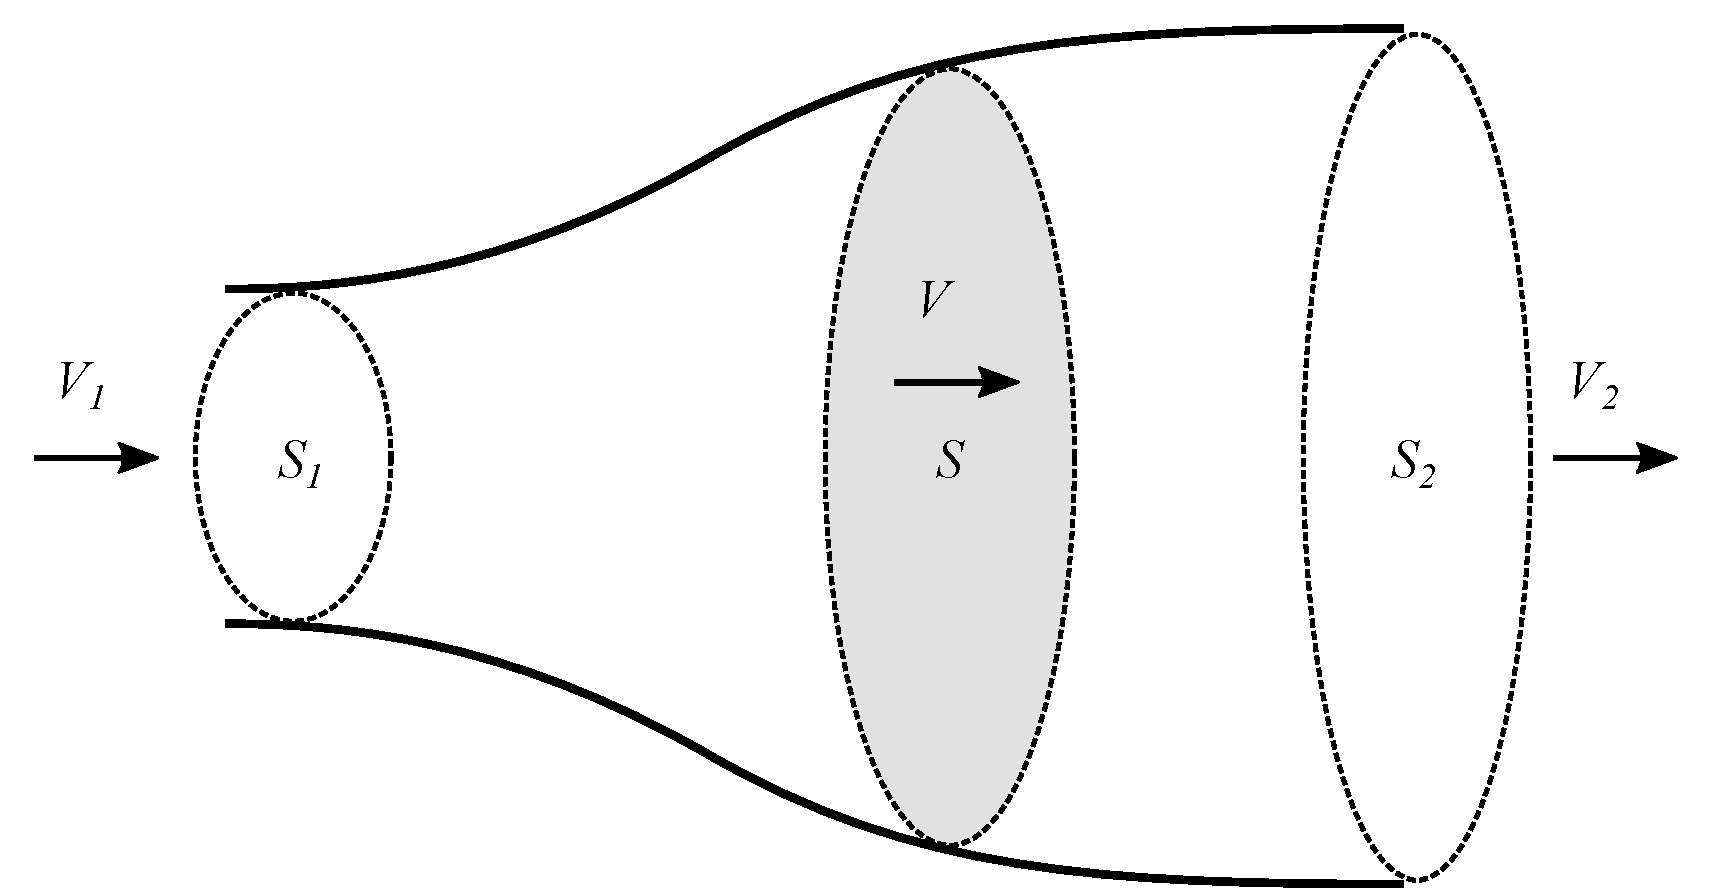
\includegraphics[width=.6\textwidth]{fig/Betz.pdf}
\caption{}
\label{}
\end{figure}
Nella realtà, il flusso a valle della turbina è vorticoso, fatto che complica molto l'analisi; l'ipotesi semplificativa di Betz consiste nell'assumere che la rotazione della turbina non trasmetta al fluido alcun moto in senso tangenziale. In ultima analisi, il flusso è bidimensionale e le sue componenti assiali e radiali. 

In virtù del Principio di Conservazione dell'Energia, se una turbina estrae una certa quantità di energia da un flusso d'aria, questo deve cedere la stessa quantità di energia cinetica. Pertanto, la velocità $V_2$ deve essere inferiore alla velocità $V_1$ visto che $S_2>S_1$:
\begin{equation}
S_1 \cdot V_1 = S_2 \cdot V_2 = S \cdot V
\end{equation}
con la sezione $S$ che indica la superficie spazzata dalla rotazione dell'elica.

Se si valuta la forza $F$ esercitata dalla turbina sul flusso d'aria in movimento, per l'equazione di Eulero, il suo valore assoluto è dato dalla seguente espressione:
\begin{equation}
F = \dot{m} \cdot \left( V_1 - V_2 \right) = S V \rho \cdot \left( V_1 - V_2 \right)
\end{equation}
con:\\[1mm]
$F$ = Valore assoluto della forza $[N]$\\
$\rho$ = densità dell'aria (da $1.2$ a $1.25$ $kg/m^3$)\\
$\dot{m}$ = portata del flusso d'aria $[kg/s]$\\
$V_1$ = velocità dell'aria a monte della turbina $[m/s]$\\
$V_2$ = velocità dell'aria a valle della turbina $[m/s]$\\
$V$ = velocità dell'aria che passa attraverso la turbina $[m/s]$\\[2mm]
La potenza P assorbita dalla turbina che viene trasferita all'albero è data da:
\begin{equation}\label{eq:potEol}
P = F \cdot V = \rho S V^2 \cdot \left( V_1 - V_2 \right)
\end{equation}
Se ora si considera la potenza assorbita dalla turbina come la variazione di energia cinetica $\Delta E$ della massa d'aria passante attraverso la sezione $S$ della turbina per ogni secondo, si otterrà la seguente espressione:
\begin{equation}\label{enEol}
\Delta E_c = \frac{1}{2} \rho	S V \left(V_1^2 - V_2^2 \right) = P
\end{equation}
Eguagliando \ref{enEol} con \ref{eq:potEol} si ottiene:
\begin{equation}
\rho S V^2 \left(V_1 - V_2 \right) = \frac{1}{2} \rho S V \left(V_1^2-V_2^2 \right)
\label{eq:P_a2}
\end{equation}
\begin{align}
	V \left(V_1 - V_2 \right)& = \frac{1}{2} \left(V_1^2-V_2^2 \right) = \\
	& = \frac{1}{2} \left(V_1-V_2 \right)\left(V_1+V_2 \right) \\
	\;\;\;\; \Rightarrow \;\;\;\; & V = \frac{V_1 + V_2}{2}
	\label{eq:vmedia}
\end{align}
Sostituendo la \ref{eq:vmedia} nella \ref{enEol} si ottiene la seguente espressione:
\begin{equation}\label{eq:potfin}
P = \frac{1}{4} \rho S \left( V_1 +V_2 \right) \cdot \left(V_1^2 - V_2^2 \right)
\end{equation}
Assumendo $V_1$ costante si può poi calcolare il valore di $V_2$ che massimizza la potenza:
\begin{align*}
\frac{dP}{dV_2} = \frac{1}{4} \rho S \left( V_1^2 - 2 V_1 V_2 - 3 V_2^2 \right) = 0
\end{align*}
Si tratta di un'equazione quadratica che ammette due radici: una è negativa ($V_2=-V_1 $) e perciò non ha significato fisico, l'altra è:
\begin{align*}
V_{2,ott} = \frac{V_1}{3}
\end{align*}
Sostituendo l'espressione appena ricavata nell'espressione di $P$ si ottiene la potenza massima estraibile:
\begin{equation}
\boxed{P_{max} = \frac{8}{27} \rho S V_1^3 = \frac{16}{27} \bigg(\frac{1}{2} \rho S V_1^3\bigg)}
\end{equation}
Questo significa che dalla potenza disponibile nel vento, rappresentata dal termine tra parentesi, fisicamente è possibile estrarne solo il 59\% ($\frac{16}{27}=0,59$); questo viene detto limite di Betz. Esso rappresenta comunque un limite teorico perchè in realtà la quota di energia che è possibile estrarre è ancora minore.

\section{Definizione del problema}
L'aria passando attraverso una turbina eolica in movimento perde velocità nel verso del flusso e, per questo motivo, le turbine devono essere sufficientemente distanziate tra loro.\\
Siccome le turbine degli aerogeneratori sono sprovviste di alette direzionali o deflettori, il movimento di rotazione delle pale genera una componente tangenziale nel moto dell'aria che porta all'innestarsi di una corrente elicoidale a valle della turbina. L'espansione del flusso genera invece una componente radiale che è stato dimostrato essere trascurabile.\\
Per la progettazione di una mini o microturbina eolica ci si può avvalere di una teoria semplificata la cui validità è stata dimostrata per via empirica. Si effettuano le seguenti ipotesi di lavoro:
\begin{enumerate}
\item le condizioni indisturbate a monte della turbina sono velocità $V_1$ e pressione $p_0$;
\item le condizioni asintotiche a valle della turbina sono velocità $V_2$ ($<V_1$), pressione $p_0$ e moto rotazionale con velocità angolare $\omega$;
\item un infinitesimo a monte del piano di rotazione della turbina, la pressione è $p$, la velocità sull'asse delle $x$ è $V$ e la rotazione delle pale con velocità angolare $\Omega$ induce sull'aria un moto rotazionale con la stessa velocità angolare;
\item un infinitesimo a valle del piano di rotazione della turbina, la pressione è $p_1$ e la velocità sull'asse delle $x$ è sempre $V$, ma il moto rotazionale indotto sull'aria ha una velocità angolare pari a $\Omega+\omega$;
\item si analizzano i flussi d'aria attraverso un'area differenziale $dS$, situata ad una distanza generica $r$ dall'asse di rotazione della turbina; lo spessore di questo anello differenziale è $dr$.
\end{enumerate}
\begin{figure}
\centering
  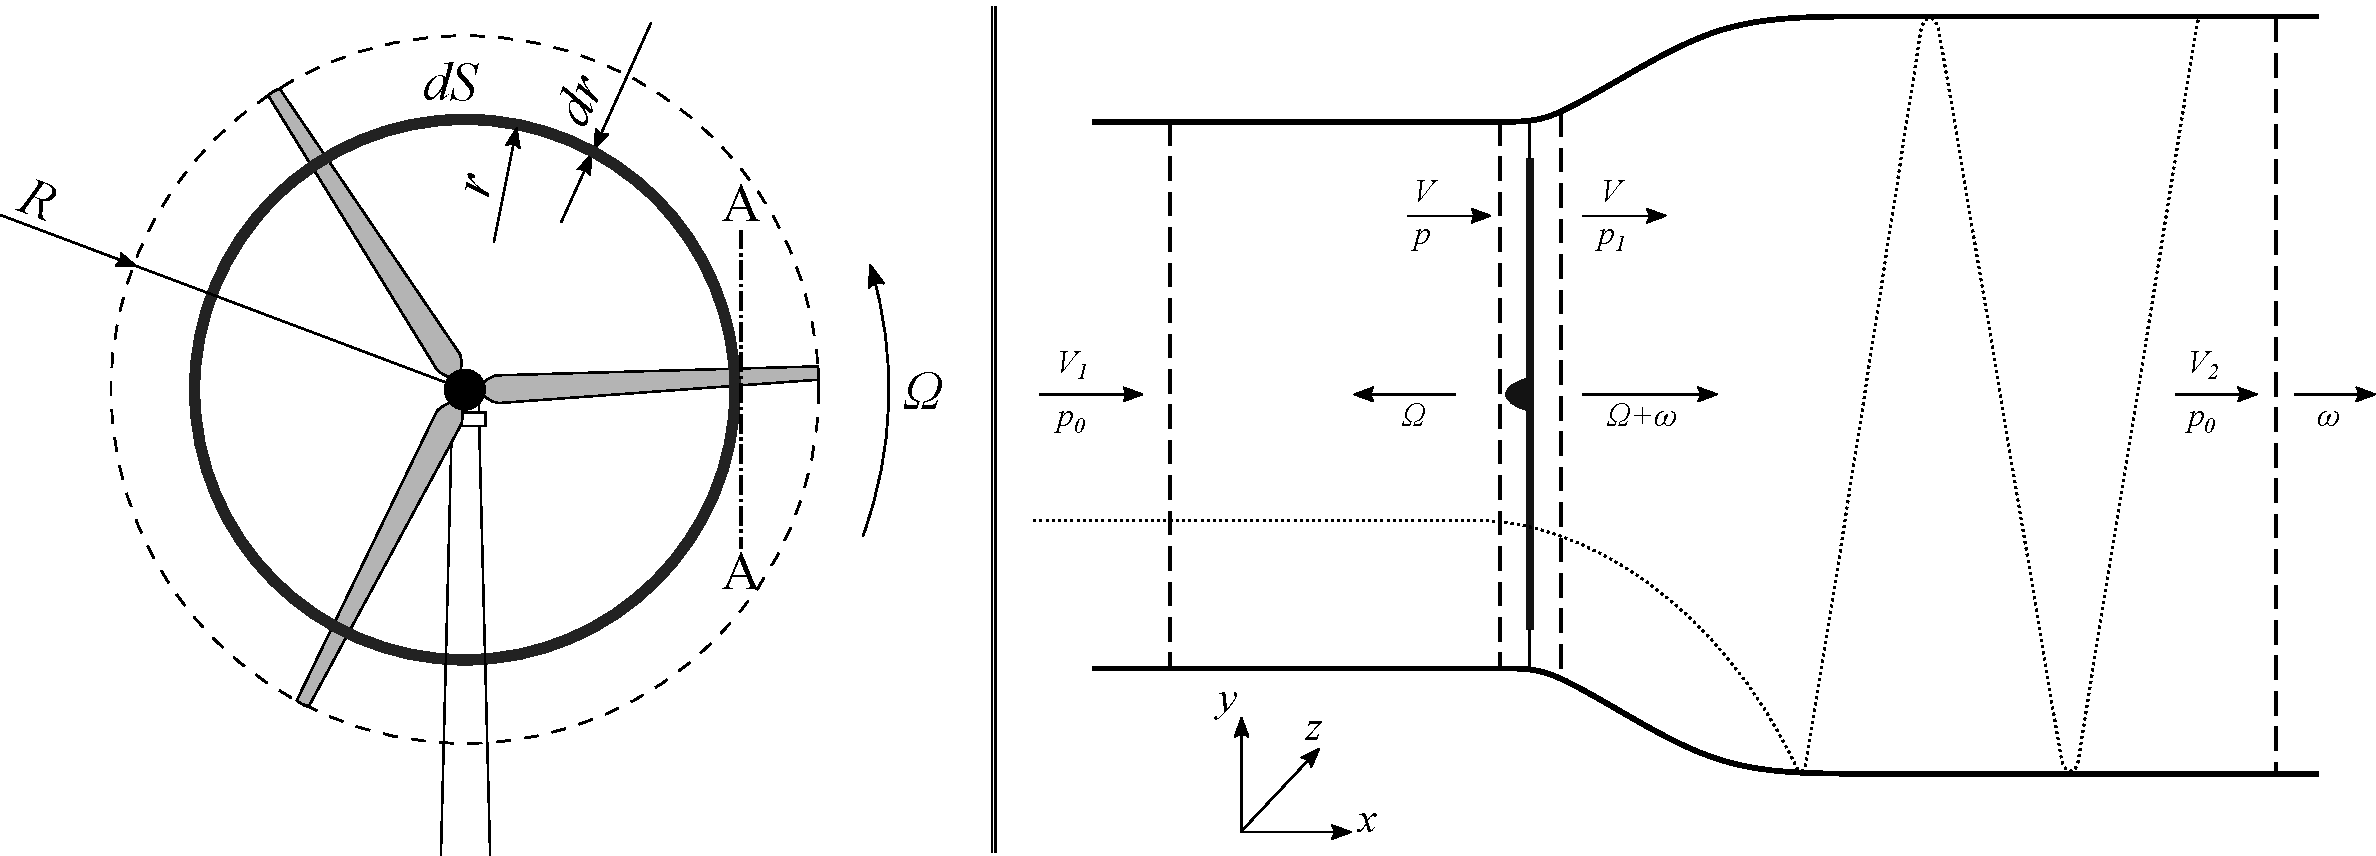
\includegraphics[width=\textwidth]{fig/frontlatEol.pdf}
\caption{A sinistra la turbina vista dal lato monte, a destra la vista laterale.}
\label{fig:frontlatEol}
\end{figure}
\begin{figure}
\centering
  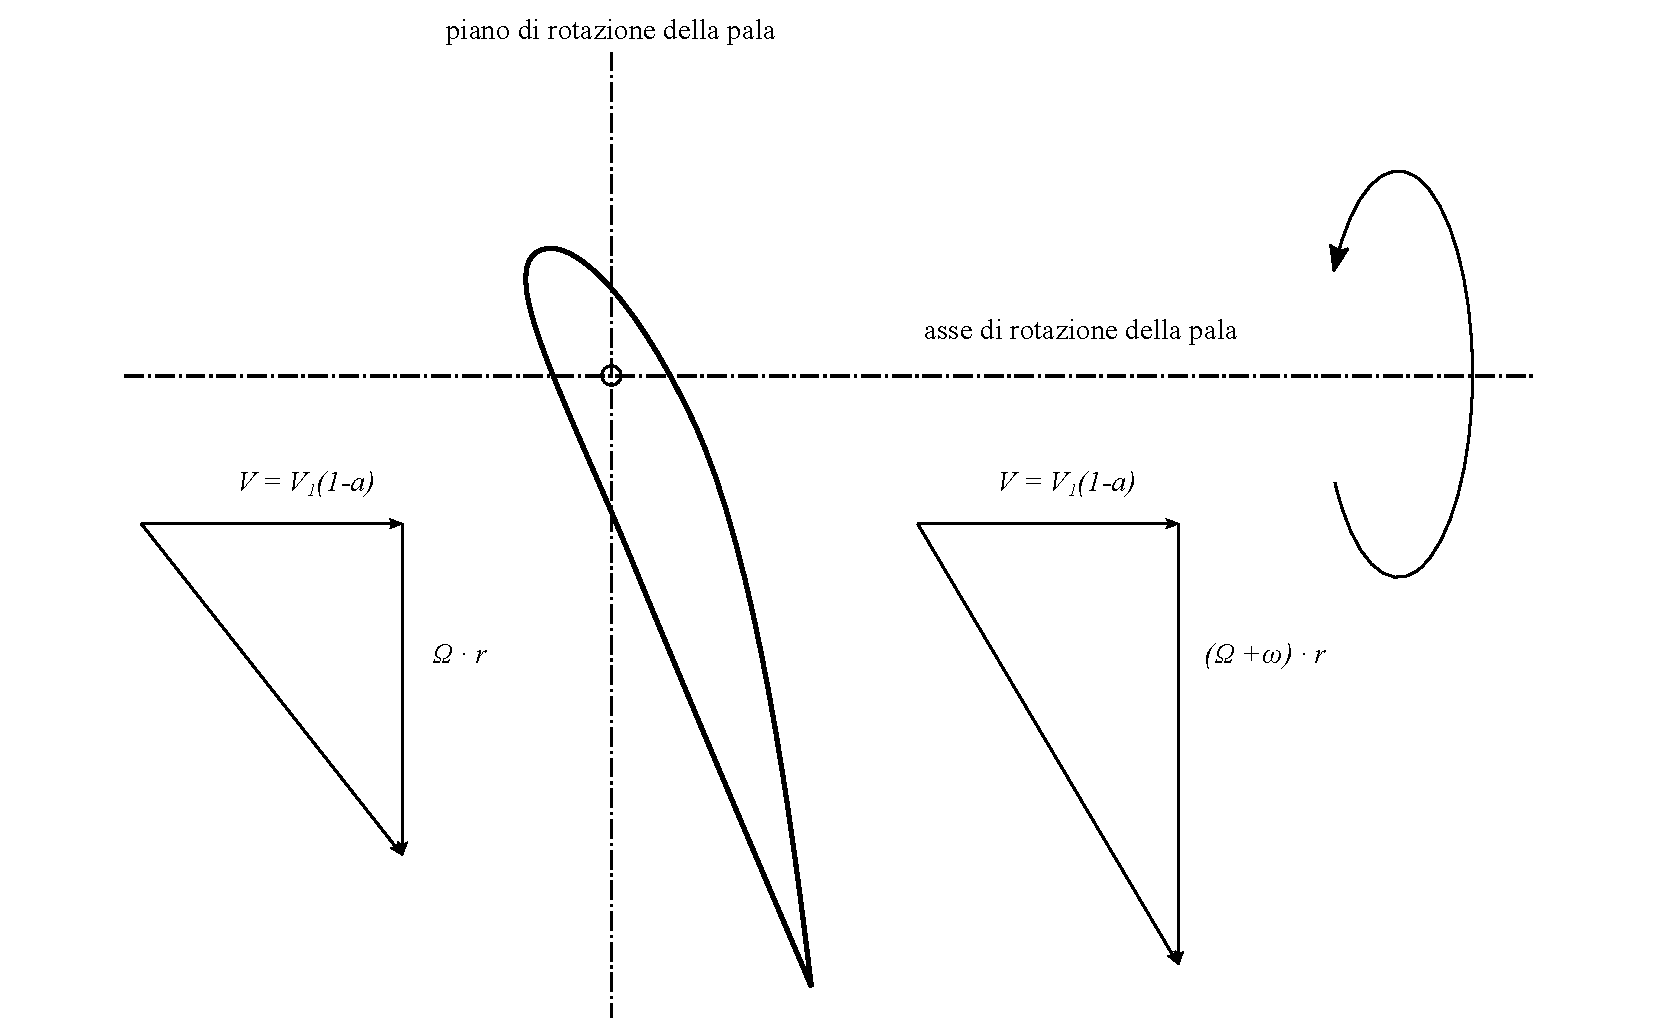
\includegraphics[width=\textwidth]{fig/triangEol.pdf}
\caption{Composizione delle velocità in un elemento di pala generico dell'elica in movimento (corrispondente alla sezione A-A della figura \ref{fig:frontlatEol}). $a$ rappresenta il coefficiente di riduzione della velocità nell'attraversamento della turbina.}
\label{fig:triangEol}
\end{figure}
Si possono definire una serie di parametri caratteristici relativi alla turbina eolica:\\[1mm]
\textbf{Solidità}: $\sigma=\cfrac{A}{S}$ , rapporto tra somma delle aree delle pale e area spazzata dalle pale.\\
\textbf{Coefficiente di velocità specifica locale}: $\lambda=\cfrac{u}{V_1}=\cfrac{\Omega \cdot R}{V_1}$ , lo stesso coefficiente per un punto $r$ generico si può esprimere in funzione di $\lambda$: $\lambda_r = \cfrac{\Omega \cdot r}{V_1} = \cfrac{\lambda \cdot r}{R}$ .\\
\textbf{Coefficiente di coppia motrice}: $c_M=\cfrac{2M}{\rho S R V_\infty^2}$ con M momento trasmesso all'albero.\\
\textbf{Coefficiente di spinta assiale}: $c_F=\cfrac{2F}{\rho S V_\infty^2}$ con F forza assiale che agisce sulla macchina.\\
\textbf{Cifra di potenza}: $c_P=\cfrac{2P}{\rho S V_\infty^3}$ , visto che $P = F \cdot V = M\cdot \Omega$ si può dire che $c_P=c_F=c_M \cdot \lambda$.\\
\textbf{Coefficiente di perdita di velocità}: $a=1-\cfrac{V}{V_1}$ , esso consente di esprimere $V$ in funzione della velocità del vento a monte della pala $V=V_1 (1-a)$; uguagliando questa equazione con la \ref{eq:vmedia}:
\begin{align*}
V_1 (1-a) = \frac{V_1 +V_2}{2} \;\;\;\; \Rightarrow \;\;\;\; 2 V_1 (1-a) - V_1 = V_2
\end{align*}
\begin{equation}\label{eq:v2}
\boxed{V_2 = V_1 (1-2a)}
\end{equation}
Il valore di $a$ non è noto a priori, si sa che deve essere $0 < a < 1/2$ e idealmente si deve avere $a = 1/3$\footnote{Dal teorema di Betz, $V_2=\frac{V_1}{3}$}. Un valore pari a $1/2$ renderebbe nulla $V_2$, condizione fisicamente impossibile. Una condizione $a=0$ implicherebbe $V_2 = V_1$ (turbina frenata).\\
\textbf{Coefficiente di velocità angolare}: $a' = \cfrac{\omega}{2 \Omega}$ , la velocità angolare della turbina è pari a $\Omega$. L'interazione delle pale del rotore con l'aria introduce su quest'ultima una componente rotazionale, la cui velocità angolare è pari a $\omega$.\\

Per calcolare la potenza sviluppata da un elemento differenziale di pala, si possono usare le equazioni di conservazione della quantità di moto; in questo modo si potrà integrare la potenza di un elemento differenziale per la lunghezza della pala e ricavare la potenza totale. Conoscendo la potenza massima ottenibile, si potranno definire in ogni punto della pala la corda e l'angolo di attacco del profilo.

\section{Teoria del tubo di flusso anulare con scia vorticosa}
Si vogliono trovare le relazioni che legano $a$, $a'$ e $\lambda$. Conoscendo tali relazioni si possono ricavare i valori di $V_1$, $V_2$ e $\omega$.\\
Facendo riferimento alla figura \ref{fig:frontlatEol} si applica il teorema di Bernoulli tra una sezione posta infinitamente a monte della turbina e una posta un infinitesimo a monte:
\begin{equation}\label{eq:bernmonte}
p_0 + \frac{\rho V_1}{2} = p + \frac{\rho V}{2}
\end{equation}
Si applica ora il teorema tra una sezione infinitesimamente a valle della turbina e una infinitamente a valle:
\begin{equation}\label{eq:bernvalle}
p_0 + \frac{\rho V_2}{2} = p_1 + \frac{\rho V}{2}
\end{equation}
Sottraendo membro a membro le equazioni \ref{eq:bernmonte} e \ref{eq:bernvalle} si ottiene:
\begin{equation}
\frac{\rho V_1^2}{2} - \frac{\rho V_2^2}{2} = p - p_1 = \Delta p
\end{equation}
Sostituendo la relazione \ref{eq:v2} tra $V_1$ e $V_2$ ed esplicitando rispetto $V_1$ \footnote{$V_2$ è ignota}:
\begin{align*}
\Delta p &= \frac{\rho}{2} \left(V_1^2 - V_2^2 \right) = \frac{\rho}{2} \left[ V_1^2 - V_1^2 \left(1-2a \right)^2 \right]=\\
&= \frac{\rho V_1^2}{2} \left[ 1- \left( 1- 2a \right)^2 \right] = \frac{\rho V_1^2}{2} \left( 1- 1+4a-4a^2 \right)=\\
&= 2 \rho V_1^2 a \left( 1-a \right)
\end{align*}
La forza esercitata dal vento sulla corona differenziale $dS$ si può dunque calcolare come:
\begin{align*}
dF_a = \Delta p \cdot dS = 2 \rho V_1^2 a \left( 1-a \right) \cdot 2 \pi r dr
\end{align*}
\begin{equation}\label{eq:forza1}
dF_a = 4 \pi \rho	V_1^2 a \left( 1-a \right) r dr
\end{equation}
Ora si applica l'equazione di Bernoulli a monte e a valle di una corona circolare di raggio $r$ e area $dS$. Dalla figura \ref{fig:triangEol} si evince che, essendo il flusso bidimensionale, vanno considerate le risultanti vettoriali di dette componenti di velocità $V_m$ e $V_v$ \footnote{I pedici indicano rispettivamente ``monte" e ``valle"}. Si ottiene:
\begin{align*}
p_1 + \frac{\rho V_m^2}{2} = p_2 + \frac{\rho V_v^2}{2}
\end{align*}
Applicando il teorema di Pitagora:
\begin{align*}
\begin{cases}
V_m^2 = V^2 + \left( \Omega r \right)^2 = V_1^2 \left(1-a \right)^2 + \left( \Omega r \right)^2\\
V_v^2 = V^2 + \left( \Omega + \omega \right)^2 r^2= V_1^2 \left(1-a \right)^2 + \left( \Omega + \omega \right)^2 r^2
\end{cases}
\end{align*}
e inserendo $V_v$ e $V_m$ nelle equazioni di Bernoulli, si ottiene:
\begin{align*}
\Delta p & =\frac{\rho}{2} \left[ V^2 + \left( \Omega + \omega \right)^2 r^2 - V^2 - \left( \Omega r \right)^2 \right]=\\
& =\frac{\rho r^2}{2} \left[ \left( \Omega + \omega \right)^2 - \Omega^2 \right]= \\
& =\frac{\rho r^2}{2} \left[ 2 \Omega \omega + \omega^2 \right]
\end{align*}
Utilizzando ora il coefficiente $a'$ precedentemente definito è possibile rimpiazzare la componente ignota $\omega$ con il suo valore in funzione della componente $\Omega$:
\begin{align*}
\Delta p &= \frac{\rho r^2}{2} \left[ 2 \Omega \left( 2 \Omega a'\right) + \left( 2 \Omega a' \right)^2 \right]=\\
&= \frac{\rho r^2}{2} \left[ 4 \Omega^2 a' + 4 \Omega^2 a'^2 \right] = \\
&= 2 \rho r^2 \Omega^2 a' \left( 1+a' \right)
\end{align*}
La spinta assiale sulla corona $dS$ vale, allora:
\begin{align*}
dF_a = \Delta p \cdot dS = 2 \rho r^2 \Omega^2 a' \left(1 + a' \right) \cdot \left( \pi 2 r dr \right)
\end{align*}
\begin{equation}\label{eq:forza2}
dF_a = 4 \pi \rho \Omega^2 a' \left( 1+ a' \right) r^3 dr
\end{equation}
Sono state ottenute due espressioni equivalenti per la forza $dF_a$: una in funzione del coefficiente $a$ e della velocità $V_1$ (\ref{eq:forza1}) e l'altra in funzione del coefficiente $a'$ e della velocità angolare $\Omega$ (\ref{eq:forza2}). Eguagliandole si ottiene:
\begin{align*}
4 \pi \rho V_1^2 a \left( 1 - a \right) r dr = 4 \pi \rho \Omega^2 a' \left( 1 + a' \right) r^3 dr
\end{align*}
\begin{align*}
V_1^2 a \left( 1 - a \right) = \Omega^2 a' \left( 1 + a' \right) r^2
\end{align*}
\begin{equation}\label{eq:lambdara}
\frac{a \left( 1 - a \right)}{a' \left(1 + a' \right)} = \frac{\Omega^2 r^2}{V_1^2}\doteq \lambda_r^2 \;\;\;\; \Rightarrow \;\;\;\; \boxed{\lambda_r^2 = \frac{a \left(1 - a \right)}{a' \left( 1 + a' \right)}}
\end{equation}
Ora che si conoscono i rapporti tra $a$, $a'$ e $\lambda_r$ si può calcolare la potenza erogata dal differenziale di pala. Dalla figura \ref{fig:triangEol} si desume che la componente assiale di velocità del vento $V$ rimane costante nell'attraversamento della pala visto che è solo la componente tangenziale a generare lavoro. Per calcolare la forza tangenziale si scrive l'impulso:
\begin{align*}
F_t = \dot{m} \cdot \Delta V
\end{align*}
Assumendo che l'aria si comporti come un fluido incompressibile, fatto che si riscontra vero nelle condizioni operative abituali di una turbina eolica, la portata di massa $\dot{m}$ che attraversa l'area $dS$ si può calcolare come 
\begin{align*}
\dot{m} = \rho V dS
\end{align*}
Quando l'aria attraversa la turbina, la componente di flusso assiale non subisce variazioni di velocità (per le ipotesi del teorema di Betz) mentre la componente di flusso tangenziale subisce una variazione di velocità:
\begin{align*}
\Delta V = \left( \Omega + \omega \right) \cdot r - \Omega \cdot r = \omega \cdot r
\end{align*}
\'E quindi possibile esprimere la forza tangenziale esercitata dall'aria sull'elemento differenziale di pala all'interno della corona di area $dS$ come:
\begin{align*}
dF_t = \rho V dS \cdot \omega r
\end{align*}
Si può dunque rimpiazzare $dS$ con la sua espressione completa e $V$ con il suo equivalente in funzione della velocità del vento nota $V_1$ utilizzando a questo scopo il coefficiente $a$:
\begin{align*}
dF_t &= \rho \left[ V_1 \left(1 -a \right) \right] \left( 2 \pi r dr \right) \cdot \omega r\\
& = 2 \pi \rho V_1 \left( 1-a \right) \omega r^2 dr
\end{align*}
Scrivendo ora la grandezza ignota $\omega$ con il suo equivalente utilizzando il coefficiente $a'$:
\begin{align*}
dF_t = 2 \pi \rho V_1 \left( 1- a \right) 2 \Omega a' r^2 dr
\end{align*}
\begin{equation}\label{eq:dftfin}
dF_t = 4 \pi \rho V_1 \left(1-a \right) \Omega a' r^2 dr
\end{equation}
La potenza generata da questa forza, per definizione, è uguale al prodotto fra il momento che produce rispetto al centro di rotazione e la sua velocità angolare, si avrà quindi:
\begin{align*}
dP &= 4 \pi \rho V_1 \left( 1-a \right) \Omega a' r^2 dr \cdot r \cdot \Omega \\
&= 4 \pi \rho V_1 \left( 1-a \right) \Omega^2 a' r^3 dr
\end{align*}
Si rimpiazza ora $\Omega^2$ per il suo equivalente in funzione di $\lambda_r$:
\begin{align*}
dP = 4 \pi \rho V_1^3 \left( 1- a \right) \frac{\lambda_r^2}{r^2} a' r^3 dr
\end{align*}
\begin{equation}\label{eq:dP}
dP = 4 \pi \rho V_1^3 \left( 1 - a \right) \lambda_r^2 a' r dr
\end{equation}
Siccome $\lambda_r > 0$, la potenza sarà massima quando il prodotto $a' \left( 1- a \right)$ sarà massimo, cioè quando la sua derivata sarà nulla ($a$ e $a'$ sono dipendenti e per questo nel calcolo della derivata si usa la regola del prodotto):
\begin{align*}
\frac{d}{da} \left( 1-a \right) a' + \left( 1 -a \right) \frac{da'}{da} = 0
\end{align*}
\begin{align*}
\left( 1- a \right) \frac{da'}{da} = a'
\end{align*}
\begin{equation}\label{eq:aa'}
\left(1 - a \right) da' = a' da
\end{equation}
$a$ e $a'$ sono legate dall'equazione \ref{eq:lambdara} che si può riscrivere come:
\begin{equation}\label{eq:lambdaraa'}
\lambda_r^2 \cdot a' \left( 1+ a' \right) = a \left( 1 - a \right)
\end{equation}
Visto che $a'$ è funzione di $a$, è possibile differenziare membro a membro l'equazione \ref{eq:lambdaraa'} rispetto ad $a$ [utilizzando la regola della catena $D(f(g(x)))=f'(g(x))*g'(x)$]:
\begin{align*}
\lambda_r^2 \left( 1+ 2a' \right) \frac{da'}{da} = \left( 1 - 2a \right)
\end{align*}
\begin{equation}\label{eq:lambdaaa'}
\lambda_r^2 \left( 1+ 2a' \right) da' = \left( 1 - 2a \right)da
\end{equation}
Moltiplicando membro a membro la \ref{eq:aa'} e la \ref{eq:lambdaaa'} si ottiene:
\begin{align*}
\lambda_r^2 \left( 1 + 2a' \right) a' da da' = \left( 1 - 2a \right) \left( 1-a \right) da da'
\end{align*}
\begin{align*}
\lambda_r^2 \left( 1 + 2a' \right) a' = \left( 1- 2a \right) \left(1 -a \right)
\end{align*}
Rimpiazzando ora il valore $\lambda_r^2$ dall'equazione \ref{eq:lambdara} risulta:
\begin{align*}
\frac{a \left(1 - a \right)}{a' \left(1 + a' \right)} = \frac{\left( 1 - 2a \right) \left( 1 -a \right)}{\left(1 + 2a' \right) a'}
\end{align*}
\begin{align*}
\frac{a}{\left( 1 + a' \right)} = \frac{\left( 1 - 2a \right)}{\left( 1 + 2a' \right)}
\end{align*}
\begin{align*}
a + 2 a a' = 1 - 2a + a' - 2aa'
\end{align*}
\begin{align*}
4aa' -a' = 1 - 3a
\end{align*}
\begin{equation}\label{eq:finala'a}
\boxed{a' = \frac{1 - 3a}{4a -1}}
\end{equation}
Riassumendo, le equazioni \ref{eq:lambdara} e \ref{eq:finala'a} vincolano $a$, $a'$ e $\lambda$ affinché la potenza estratta sia massima.\\
Si rimpiazza ora $r$ nell'equazione \ref{eq:dP} esprimendolo in funzione di $\lambda_r$ (vedi la definizione di $\lambda_r$):
\begin{align*}
dP = 4 \pi \rho V_1^3 a' \left( 1 - a \right) \lambda_r^2 \frac{R \lambda_r}{\lambda} dr
\end{align*}
Si può poi sostituire $dr$ come segue
\begin{align*}
\frac{dr}{d \lambda_r} = \frac{R}{\lambda} \;\;\;\; \Rightarrow \;\;\;\; dr = \frac{R}{\lambda} d \lambda_r
\end{align*}
\begin{align*}
dP &= 4 \pi \rho V_1^3 a' \left(1 - a \right) \lambda_r^2 \frac{R \lambda_r}{\lambda} \frac{R}{\lambda} d \lambda_r\\
&= 4 \pi \rho V_1^3 \frac{R^2}{\lambda^2} a' \left( 1 - a \right) \lambda_r^3 d\lambda_r
\end{align*}
A questo punto è possibile ottenere la potenza totale prodotta dalla turbina integrando tra $\lambda_r = 0$ (centro del rotore) e $\lambda_r = \lambda$ (estremità della pala):
\begin{align*}
P = 4 \pi \rho V_1^3 \frac{R^2}{\lambda^2} \int_0^{\lambda} a' \left( 1 - a \right) \lambda_r^3 d \lambda_r
\end{align*}
In queste condizioni il coefficiente di potenza $c_P$ vale:
\begin{align*}
c_P = \cfrac{P}{\cfrac{\rho}{2} \pi R^2 V_1^3} = \cfrac{4 \pi \rho V_1^3 R^2}{\cfrac{\rho}{2} \pi R^2  V_1^3 \lambda^2} \int_0^{\lambda} a' \left(1 - a \right) \lambda_r^3 d \lambda_r
\end{align*}
\begin{equation}
c_P = \frac{8}{\lambda^2} \int_0^{\lambda} a' \left( 1 - a \right) \lambda_r^3 d \lambda_r
\end{equation}
Quest'ultimo integrale è detto integrale di Glauert; esso è estremamente difficile da risolvere per via algebrica e perciò la soluzione deve essere ricavata per via numerica.
\begin{figure}[h!]
\centering
  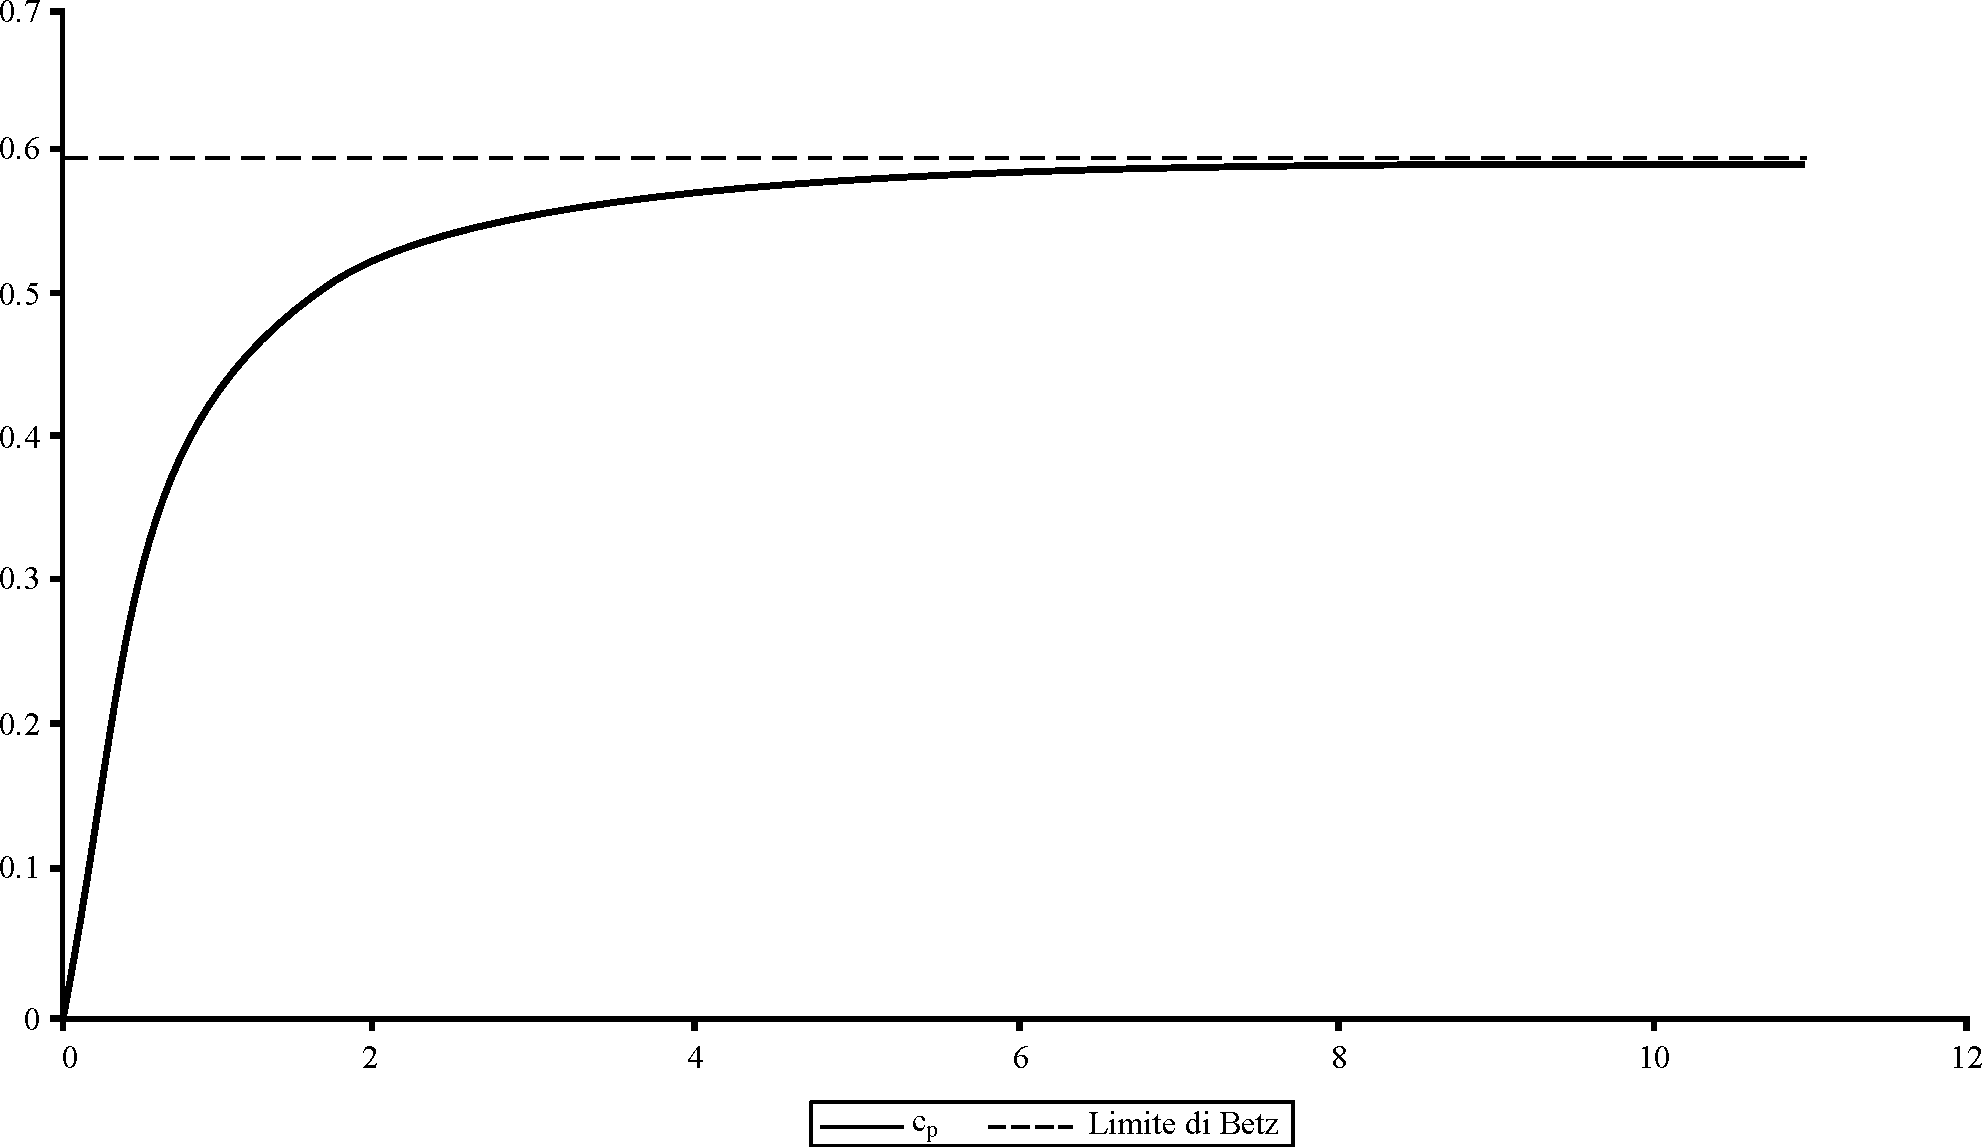
\includegraphics[width=.7\textwidth]{fig/limBetz.pdf}
\caption{In ascissa è presente $\lambda$}
\label{fig:limBetz}
\end{figure}
La teoria di Glauert evidenzia che il rendimento aerodinamico cresce con $\lambda$ e si avvicina in modo asintotico al limite di Betz. \\
Con questa teoria non ancora possibile progettare una pala, ma le espressioni ottenute in precedenza servono a definire le condizioni al contorno che ogni elemento di pala deve soddisfare affinché la pala, nel suo insieme, risulti ottima.

\section{Forze aerodinamiche sull'elemento di pala}
Ora verrà affrontata la progettazione delle pale dal punto di vista delle forze aerodinamiche agenti sull'elemento differenziale della pala già definito nella figura \ref{fig:frontlatEol}. 

Risulta doveroso fare una premessa: nella progettazione di turbine commerciali di grande taglia generalmente si utilizzano modelli di calcolo più sofisticati di quello che verrà esposto.
Poiché i profili delle pale delle turbine di piccola potenza operano in condizioni di basso Re e visto che in prossimità del suolo il profilo di velocità del vento è irregolare, non ha senso basare il progetto delle pale su teorie più complesse. La validità del metodo descritto di seguito è stata comunque verificata in galleria del vento, ma per maggiori approfondimenti si faccia riferimento alla bibliografia del libro citato all'inizio di questo capitolo.

Si osserva la figura \ref{fig:frontlatEol}; l'esperienza insegna che un elemento di pala compreso tra due raggi $r$ e $r+dr$ in presenza di una corrente di aria, sarà sottoposto ad un complesso di forze le quali dipenderanno dalla forma del profilo della pala e dall'angolo d'incidenza tra la corda del profilo e la velocità relativa dell'aria $W$.
\begin{figure}[h!]
\centering
  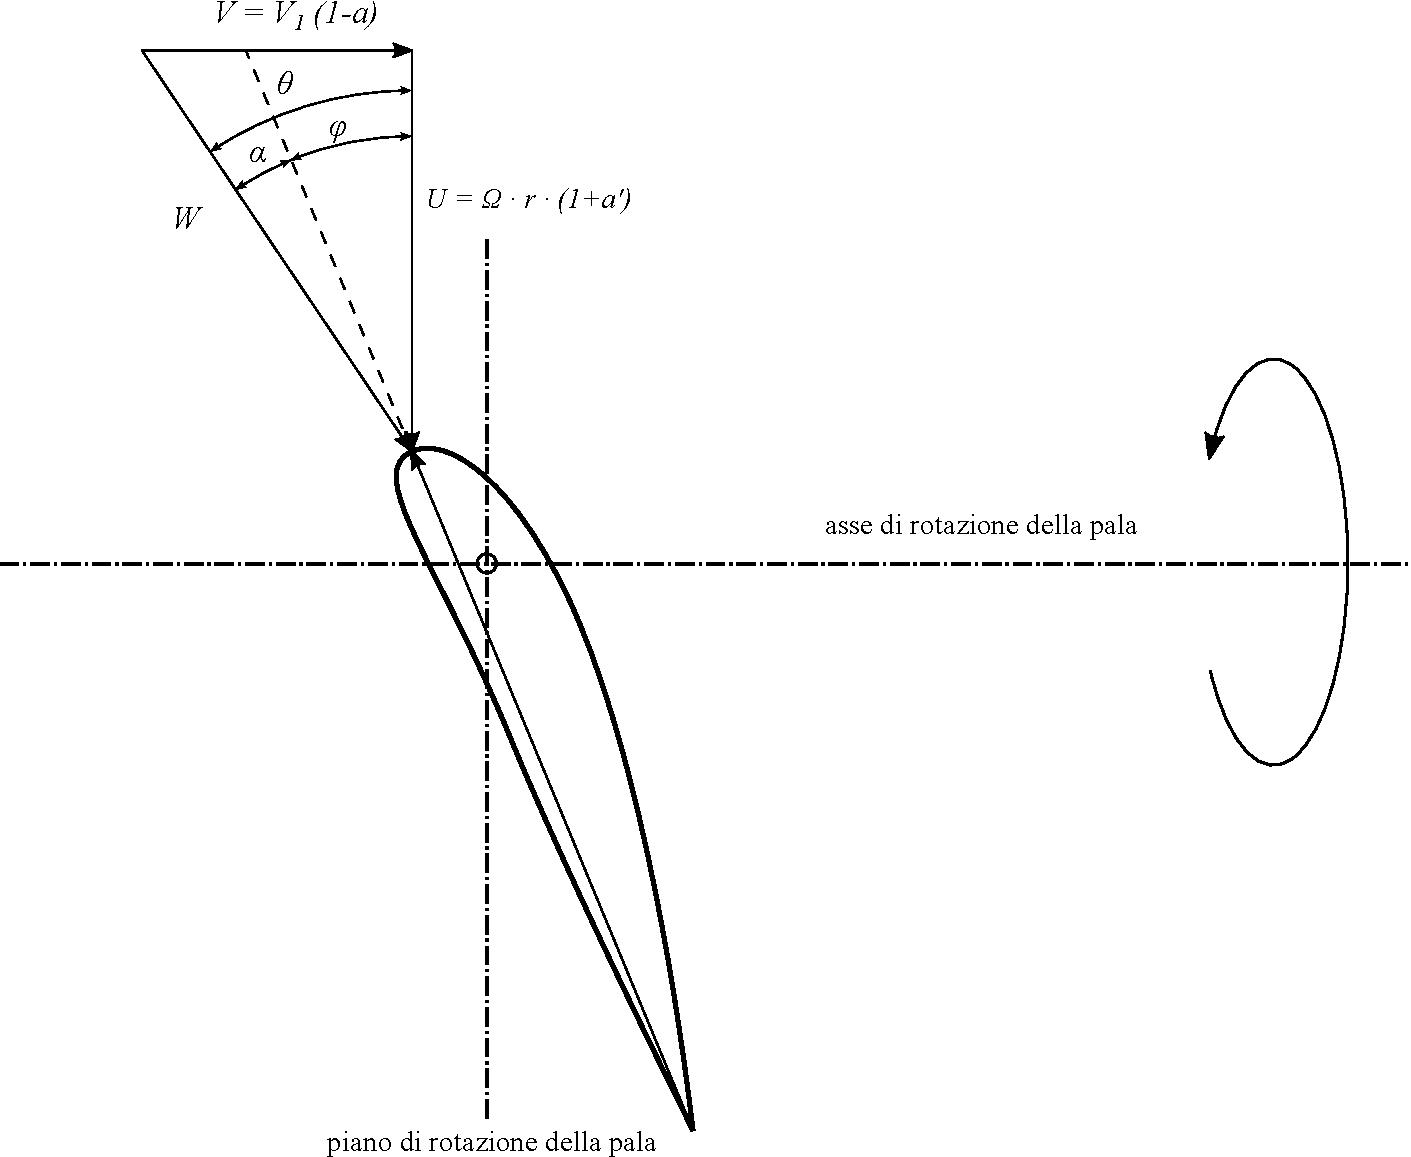
\includegraphics[width=.7\textwidth]{fig/triangEol2.pdf}
\caption{}
\label{fig:triangEol2}
\end{figure}
\\ Nella figura \ref{fig:triangEol2} si osservano le velocità relative tra la pala e l'aria, derivate dalla figura \ref{fig:triangEol} e dalla teoria di Glauert trattata precedentemente. Gli angoli indicati in figura \ref{fig:triangEol2} si definiscono come:
\begin{itemize}
	\item $\alpha$: angolo d'incidenza sulla sezione del profilo rispetto la corda del profilo;
	\item $\varphi$: angolo di calettamento della sezione del profilo o passo locale dell'elica rispetto la corda del profilo;
	\item $\theta$: angolo fra il piano di rotazione della pala e la velocità relativa $W$. Dalla figura si deduce che $\theta = \alpha + \varphi$.
\end{itemize}
Inoltre, osservando il triangolo delle velocità, vale:
\begin{equation}\label{eq:tantheta}
\tan \theta = \frac{V_1 \left(1-a \right)}{\Omega r \left(1 + a' \right)} = \frac{\left( 1-a \right)}{\lambda \left( 1 + a' \right)}
\end{equation}
\begin{equation}
	W^2 = U^2 + V^2 = V_1^2 \left(1-a \right)^2 + \Omega^2 r^2 \left( 1+ a' \right)^2
\end{equation}
La velocità relativa $W$, incidendo sul profilo con angolo $\alpha$, genera le seguenti forze aerodinamiche:
\begin{itemize}
	\item \textbf{portanza}: $dF_z = \cfrac{\rho}{2} C_z l W^2 dr$
	\item \textbf{resistenza o forza di trascinamento}: $dF_x = \cfrac{\rho}{2} C_x l W^2 dr$
\end{itemize}
con $l$ lunghezza della corda del profilo, per ora incognita.\\
L'obiettivo è determinare quale deve essere il valore ottimale di $l$ per una data coppia di valori $C_z$ e $C_x$ scelti dalla curva delle caratteristiche del profilo alare che si vuole determinare. 
\begin{figure}[h!]
\centering
  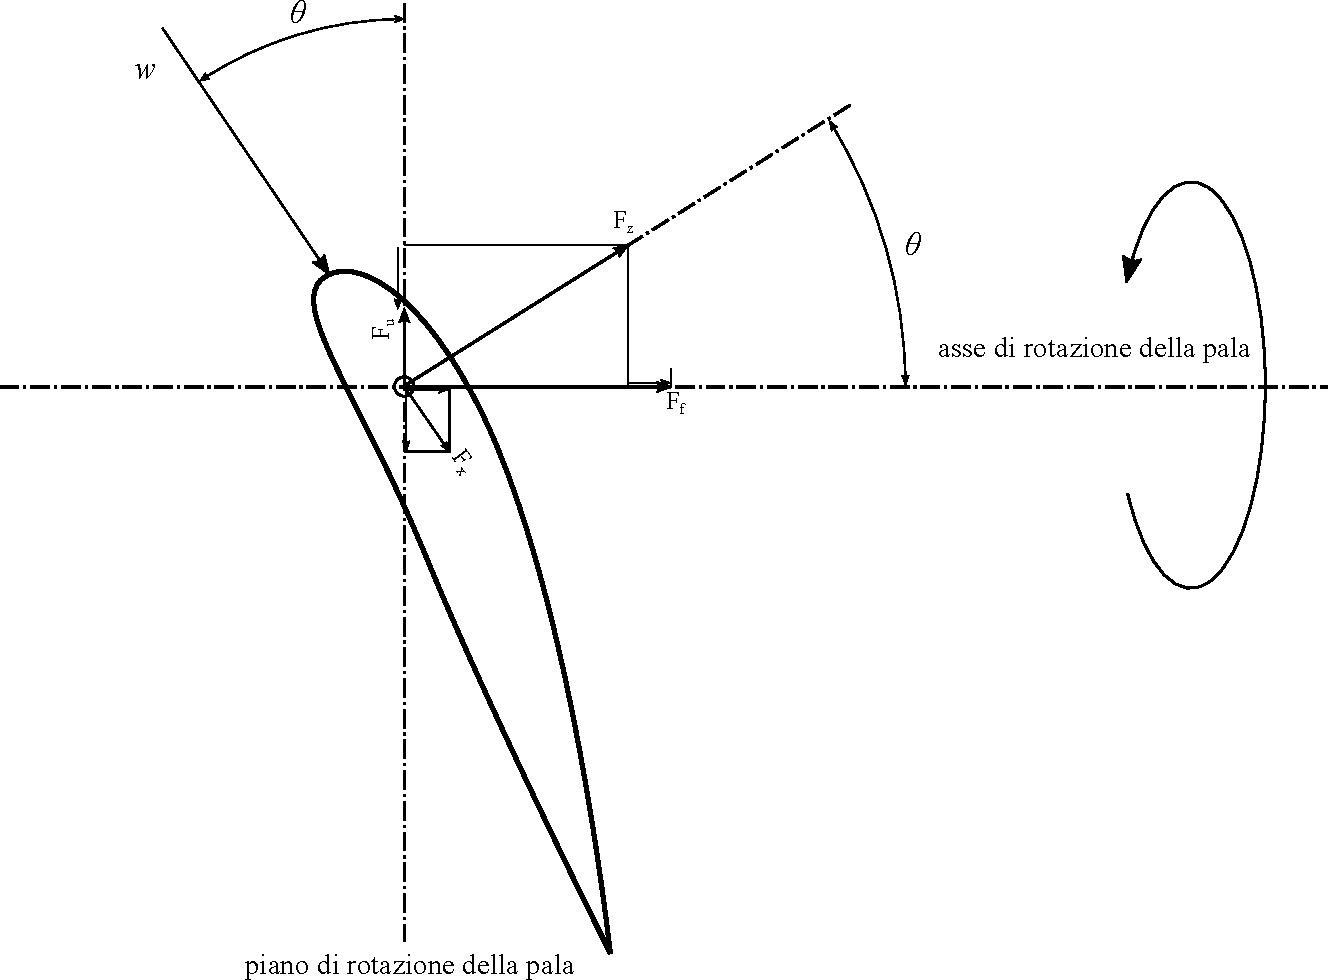
\includegraphics[width=.9\textwidth]{fig/forzeEol.pdf}
\caption{}
\label{fig:forzeEol}
\end{figure}
\\La figura \ref{fig:forzeEol} mostra le forze $F_z$ e $F_x$ rispettivamente perpendicolare e coassiale alla velocità relativa $W$. Sono inoltre evidenziate le loro proiezioni:
\begin{itemize}
	\item in senso assiale $F_f$: forza che genera soltanto sforzo di flessione sulla pala, ma non produce lavoro utile;
	\item tangenziale $F_u$: forza che genera lavoro utile.
\end{itemize}
Nel riferirsi all'elemento di pala, si chiameranno queste forze rispettivamente $dF_f$ e $dF_u$. Dalla trigonometria elementare, è possibile scrivere il valore di $dF_u$ come:
\begin{align*}
dF_u = dF_z \cdot \sin \theta - dF_x \cdot \cos \theta
\end{align*}
\begin{equation}\label{eq:dF_u1}
dF_u = \frac{\rho}{2} C_z l W^2 dr \cdot \sin \theta - \frac{\rho}{2} C_x l W^2 dr \cdot \cos \theta
\end{equation}
Con lo stesso ragionamento, si può scrivere:
\begin{equation}\label{eq:dF_f1}
dF_f = \frac{\rho}{2} C_z l W^2 dr \cdot \cos \theta + \frac{\rho}{2} C_x l W^2 dr \cdot \sin \theta
\end{equation}
In un profilo alare operante in condizioni ottimali, si ha sempre che $C_z \gg C_x$; per questo motivo le equazioni \ref{eq:dF_u1} e \ref{eq:dF_f1} possono essere semplificate come segue:
\begin{equation}\label{eq:dF_u2}
dF_u \approx \frac{\rho}{2} C_zl W^2 dr \sin \theta
\end{equation}
\begin{equation}\label{eq:dF_f2}
dF_f \approx \frac{\rho}{2} C_zl W^2 dr \cos \theta
\end{equation}
Se il numero di pale è pari a $z$, si può scrivere che la forza assiale $dF_a$ sulla corona differenziale di pala è:
\begin{align*}
dF_a = \frac{\rho}{2} z C_z l W^2 dr \cos \theta
\end{align*}
Si rimpiazza $W^2$ con il suo valore in funzione di $\theta$:
\begin{equation}\label{eq:dFa}
dF_a = \frac{\rho}{2} z C_z l \frac{V_1^2 \left( 1- a \right)^2}{\sin^2 \theta} dr \cos \theta
\end{equation}
Se si uguagliano le espressioni \ref{eq:dFa} e \ref{eq:forza1} per la forza assiale si ottiene:
\begin{align*}
4 \pi \rho V_1^2 a \left( 1-a \right) r dr = \frac{\rho}{2} z C_z l \frac{V_1^2 \left( 1- a \right)^2 }{\sin^2 \theta} dr \cos \theta
\end{align*}
\begin{align*}
4 a = \frac{z l }{2 \pi r} C_z \frac{\left( 1- a \right)}{\sin^2 \theta} \cos \theta
\end{align*}
Si definisce il coefficiente di solidità locale per un elemento differenziale di turbina come:
\begin{align*}
\sigma_l = \frac{z l}{2 \pi r}
\end{align*}
Pertanto si può scrivere:
\begin{equation}\label{eq:asolid}
\cfrac{a}{1-a} = \cfrac{\sigma_l C_z \cos \theta}{4 \sin^2 \theta}
\end{equation}
La forza utile $dF_u$ genera un momento torcente rispetto all'asse di rotazione. Imponendo il numero di pale $z$ si calcola la coppia motrice differenziale totale:
\begin{equation}\label{eq:dM}
dM = z \cdot r \cdot dF_u
\end{equation}
Dall'espressione \ref{eq:dftfin} della forza tangenziale $F_t$ si può scrivere:
\begin{align*}
dM = dF_t \cdot r = 4 \pi \rho V_1 \left( 1- a \right) \Omega a' r^3 dr
\end{align*}
e uguagliando questa espressione con l'equazione \ref{eq:dM}, si ottiene:
\begin{align*}
4 \pi \rho V_1 \left(1-a \right) \Omega a' r^3 dr = z \cdot r \cdot dF_u
\end{align*}
Rimpiazzando l'espressione di $dF_u$ secondo l'equazione \ref{eq:dF_u2} nell'equazione precedente, risulta:
\begin{align*}
4 \pi \rho V_1 \left(1-a \right) \Omega a' r^3 dr = z \cdot r \cdot C_z \cfrac{\rho}{2} l W^2 dr \sin \theta
\end{align*}
Semplificando:
\begin{align*}
4 V_1 \left(1-a \right) \Omega a' r = C_z \cfrac{z l }{2 \pi r} W^2 \sin \theta
\end{align*}
Rimpiazzando $W^2$ con il suo equivalente trigonometrico ricavato dalla figura \ref{fig:triangEol2} e introducendo $\sigma_l$:
\begin{align*}
4 V_1 \left(1-a \right) \Omega a' r = \sigma_l C_z \cfrac{V_1^2 \left(1-a \right)^2}{\sin^2 \theta} \sin \theta
\end{align*}
\begin{align*}
4 \Omega a' r = \sigma_l C_z \cfrac{V_1 \left(1-a \right)}{\sin \theta}
\end{align*}
\begin{align*}
a'= \sigma_l C_z \cfrac{V_1 \left(1-a \right)}{4 \Omega r \sin \theta}
\end{align*}
Introducendo al posto di $V_1 \left(1-a\right)$ il suo equivalente trigonometrico secondo l'equazione \ref{eq:tantheta}:
\begin{align*}
a' = \sigma_l C_z \cfrac{\Omega r \left(1+a' \right) \tan \theta}{4 \Omega r \sin \theta}
\end{align*}
\begin{align*}
\cfrac{a'}{1+a'} = \sigma_l C_z \cfrac{\tan \theta}{4 \sin \theta}
\end{align*}
\begin{equation}\label{eq:aprimofin}
\cfrac{a'}{1+a'} = \cfrac{\sigma_l C_z}{4 \cos \theta}
\end{equation}
Se nell'equazione \ref{eq:aprimofin} si rimpiazza $a'$ con il suo equivalente secondo l'equazione \ref{eq:finala'a} si ottiene:
\begin{align*}
\cfrac{\cfrac{1-3a}{4a-1}}{1+\cfrac{1-3a}{4a-1}} = \cfrac{\sigma_l C_z}{4 \cos \theta}
\end{align*}
\begin{align*}
\cfrac{1-3a}{4a-1+1-3a} = \cfrac{\sigma_l C_z}{4 \cos \theta}
\end{align*}
\begin{align*}
\cfrac{1-3a}{a} = \cfrac{\sigma_l C_z }{4 \cos \theta}
\end{align*}
\begin{align*}
\cfrac{1}{a} = \cfrac{\sigma_l C_z}{4 \cos \theta} + 3
\end{align*}
\begin{equation}\label{eq:afin}
a = \cfrac{4 \cos \theta}{\sigma_l C_z +12 \cos \theta}
\end{equation}
Rimpiazzando l'equazione \ref{eq:afin} nella \ref{eq:asolid} si ottiene:
\begin{align*}
\cfrac{\cfrac{4 \cos \theta}{\sigma_l C_z + 12 \cos \theta}}{\left( 1- \cfrac{4 \cos \theta}{\sigma_l C_z + 12 \cos \theta} \right)} = \cfrac{\sigma_l C_z \cos \theta}{4 \sin^2 \theta}
\end{align*}
\begin{align*}
\cfrac{\cfrac{4 \cos \theta}{\sigma_l C_z + 12 \cos \theta}}{\cfrac{\sigma_l C_z + 12 \cos \theta - 4 \cos \theta}{\sigma_l C_z + 12 \cos \theta}} = \cfrac{\sigma_l C_z \cos\theta}{4 \sin^2 \theta}
\end{align*}
\begin{align*}
\cfrac{4}{\sigma_l C_z + 8 \cos \theta} = \cfrac{\sigma_l C_z}{4 \sin^2 \theta}
\end{align*}
\begin{align*}
4 = \cfrac{\left( \sigma_l C_z \right)^2 + \sigma_l C_z 8 \cos \theta}{4 \sin^2 \theta}
\end{align*}
\begin{align*}
16 \sin^2 \theta = \left( \sigma_l C_z \right)^2 + \sigma_l C_z 8 \cos \theta
\end{align*}
Questa è un'equazione di secondo grado, nella quale l'incognita è $\sigma_l C_z$. Le due radici sono:
\begin{align*}
\sigma_l C_z = 4 \left(-1 -\cos \theta \right)
\end{align*}
\begin{equation}\label{eq:sigmazc}
\boxed{\sigma_l C_z = 4 \left(1- \cos \theta \right)}
\end{equation}
La prima non ha significato fisico poiché nell'intervallo di interesse affinché $\sigma_l C_z > 0$ dev'essere $\cos \theta > 0 $.\\
In questo modo si è ricavata un'equazione che lega direttamente la solidità locale $\sigma_l$, e quindi la corda del profilo $l$, con l'angolo $\theta$.\\
Il coefficiente $C_z$ viene scelto arbitrariamente dal progettista sulla base di determinati criteri prestazionali e il valore di $C_x$ risulta di conseguenza in quanto la loro relazione è univoca. Per esempio si può scegliere il valore ottimo, ossia $C_z$ che corrisponde al massimo del rapporto $C_z/C_x$ (massima efficienza aerodinamica del profilo). Va sottolineato però che i valori di $C_z$ e $C_x$ riscontrabili, nella letteratura aerodinamica, valgono per un profilo di lunghezza infinita.\\
In un profilo reale, e precisamente sulla punta della pala, si produce un vortice dovuto alla differenza di pressione tra l'intradosso e l'estradosso e all'assenza di una condizione al contorno che ne impedisca la formazione. Sono state proposte pale con deflettori situati sulla punta per evitare proprio questo effetto però in pratica non sono utilizzati.\\
Dalla teoria aerodinamica, l'attrito indotto dai vortici che si sviluppano sulla punta della pala si può calcolare con la formula di Oswald:
\begin{align*}
C_{xi} = \frac{C_z^2}{\pi \cdot e \cdot AR}
\end{align*}
con:\\[1mm]
$C_{xi}$: coefficiente di resistenza indotta dai vortici;\\
$C_z$: coefficiente di portanza (da tabelle aerodinamiche per profili infiniti);\\
$e$: fattore di Oswald ($0.85 \div 0.9$ per le pale molto allungate);\\
$AR$: Aspect Ratio ($L/l$) con $L$ lunghezza totale della pala (dall'attaccatura con il mozzo fino all'estremità) e $l$ corda media della pala.\\[2mm]
Nella pratica, si dovrà considerare il valore di $C_z$ ricavato dalle tabelle di dati aerodinamici e il valore reale di resistenza aerodinamica $C_{xr}$ ricavato con
\begin{align*}
C_{xr} = C_x + C_{xi}
\end{align*}
A questo punto sono stati definiti tutti gli elementi necessari per progettare ogni sezione della pala; ciò nonostante le considerazioni esposte nei paragrafi successivi aiuteranno nella definizione dei criteri progettuali.

\subsection{Variazione ottimale di $\theta$}
Poiché in ogni posizione $r$ della pala si desidera estrarre il massimo di energia dal vento, ne consegue che $a$ e $a'$ devono soddisfare la definizione di $\lambda_r$ ($\lambda_r = \frac{\lambda \cdot r}{R}$) e di $a'$ ($a' = \frac{1 - 3a}{4a -1}$).\\
Poiché per l'angolo $\theta$ vale la relazione \ref{eq:tantheta}, ne consegue che $\theta$ è funzione di $\lambda_r$. Allo stesso modo con cui è stato tabulato il coefficiente di potenza locale in funzione di $a$, $a'$ e $\lambda_r$, si calcola l'angolo $\theta$ ottimale in ogni posizione $r$ della pala. La figura \ref{fig:lambdatheta} mostra come varia $\theta$ in funzione di $\lambda_r$.
\begin{figure}[h!]
\centering
  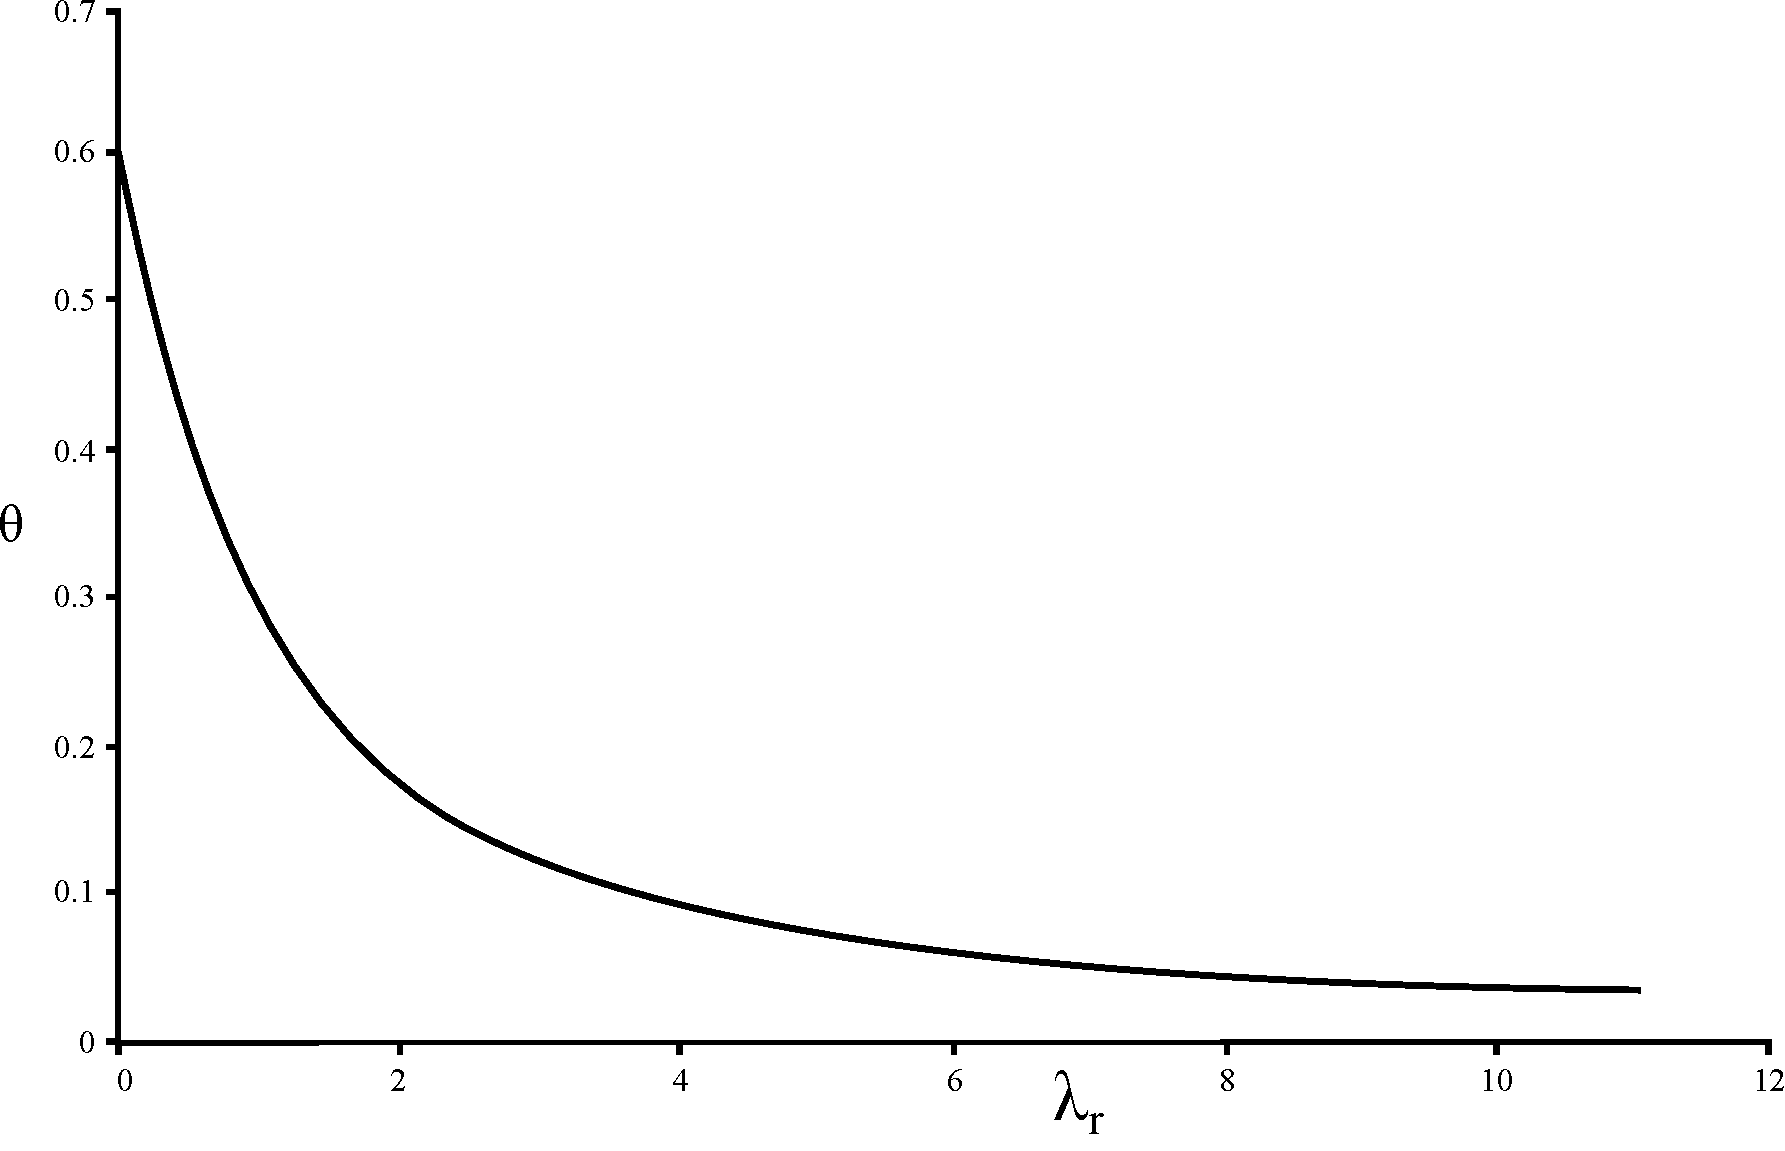
\includegraphics[width=.7\textwidth]{fig/lambdatheta.pdf}
\caption{}
\label{fig:lambdatheta}
\end{figure}
\\La curva si può rappresentare con la seguente funzione matematica equivalente, più semplice da utilizzare:
\begin{equation}
\theta = \frac{2}{3} \arctan \left( \frac{1}{\lambda_r} \right)
\end{equation}
Come è possibile notare dall'equazione \ref{eq:sigmazc} il prodotto $\sigma_l C_z$ dipende solo da $\theta$; quindi, una volta noto il valore ottimale di $\theta$, per ogni valore di $\lambda_r$ e definiti i valori di $R$ e di $\lambda$, si riesce a calcolare il prodotto $\sigma_l C_z$ sempre utilizzando l'equazione \ref{eq:sigmazc}.\\
\\
\textit{Gli argomenti da questo punto in poi non sono stati trattati direttamente a lezione nell'a.a. 2019-2020 ma sono presenti sul libro di riferimento}.\\
\\
A questo punto, definiamo ad esempio un valore di corda $l$, costante lungo  tutta la pala, e calcoliamo di conseguenza $\sigma_l$ per ogni valore di $r$, secondo la definizione della solidità locale:
\begin{align*}
\sigma_l = \frac{z l}{2 \pi r}
\end{align*}
Noto $\sigma_l$, possiamo dunque in ogni punto della pala ricavare il valore di $C_z$ necessario a soddisfare l'equazione \ref{eq:sigmazc}. Una volta noto $C_z$, dalle caratteristiche del profilo possiamo ricavare l'angolo di incidenza $\alpha$ e dunque definire il passo della sezione della pala nel punto $r_l$ cioè corrispondente all'angolo $\varphi$ della figura \ref{fig:triangEol2}. Dal punto di vista pratico, questo approccio è utile, ad esempio, per realizzare una pala a partire da un profilo estruso: affinché la corda si mantenga costante lungo la pala il profilo dovrà essere deformato mediante uno sforzo di torsione tale che l'angolo $\varphi$, in ogni punto, sia pari a quello risultante dalle equazioni:
\begin{align*}
\theta = \alpha + \varphi
\end{align*}
\begin{align*}
\theta = \frac{2}{3} \arctan \left( \frac{1}{\lambda_r} \right)
\end{align*}
\begin{align*}
\alpha = \alpha' - \beta
\end{align*}
\begin{align*}
\beta = \arctan \left( \frac{C_z \pi l}{R} \right)
\end{align*}
Una pala progettata con questo criterio è sub-ottimale, in quanto il valore di $C_z$ e l'angolo d'incidenza che ne risultano, in genere non coincideranno con il punto di massima efficienza aerodinamica del profilo, quindi non soddisfano pienamente l'ipotesi assunta per postulare le equazioni \ref{eq:dF_u2} e \ref{eq:dF_f2}, sulle quali si basa tutto il modello matematico presentato precedentemente.

\subsection{Variazione ottimale del prodotto $\sigma_l C_z$}
Come abbiamo visto, nell'equazione \ref{eq:sigmazc}, il prodotto $\sigma_l C_z$ dipende solo da $\cos \theta$ e pertanto: noto il valore ottimale di $\theta$ per ogni valore di $\lambda_r$ e avendo predefinito i valori di progetto $R$ e $\lambda$, possiamo calcolare il prodotto $\sigma_l C_z$ direttamente con l'equazione \ref{eq:sigmazc}. Se volessimo, ad esempio, costruire una pala a partire da una semplice tavola di legno (quindi senza svergolamento) innanzitutto dovremmo definire arbitrariamente un valore costante per l'angolo $\varphi$ della figura \ref{fig:triangEol2}. Definito l'angolo $\varphi$ e noto in ogni punto $r$ della pala l'angolo $\theta$, ricavato dall'equazione \ref{eq:tantheta}, è immediato calcolare l'angolo di incidenza $\alpha$. Noto $\alpha$, di conseguenza si ricava $C_z$ dalle caratteristiche del profilo, ed essendo noto il prodotto $\sigma_l C_z$, risulta immediato calcolare la corda $l$ in ogni sezione della pala.

\subsection{Pala ottimale con massima efficienza aerodinamica}
Il coefficiente di finezza $f$ dato dal rapporto $C_z/C_x$, rappresenta l'efficienza aerodinamica di un profilo. Nei paragrafi precedenti abbiamo basato le nostre ipotesi di calcolo sul fatto che $C_z \gg C_x $, fatto assolutamente vero solo con valori dell'angolo d'incidenza relativamente piccoli (in genere inferiori a $5^\circ$). Il $f$ è massimo solo in un punto della polare del profilo. Possiamo dunque progettare una pala in modo che massimizzi l'energia catturata dal vento, se in ogni punto $r$ si compiono simultaneamente le condizioni delle equazioni \ref{eq:tantheta} e \ref{eq:sigmazc}, e inoltre, se si sceglie il valore di $C_z$ corrispondente al massimo $f$ in modo che siano rispettate le ipotesi delle equazioni \ref{eq:dF_u2} E \ref{eq:dF_f2} in ogni sezione della pala. La pala risultante sarà caratterizzata dunque da un certo svergolamento e anche dalla corda variabile fra la sua attaccatura e la sua estremità. Poiché $\lambda_r$ è direttamente proporzionale ad $r_l$ possiamo tabulare il prodotto $\sigma_l C_z \lambda_r$ in funzione di $\lambda_r$ il quale a sua volta è funzione di $a$ e $a'$., nello stesso modo utilizzato per disegnare la curva della figura \ref{fig:lambdatheta}. La grafica di questa funzione rappresenta, in modo adimensionale, la variazione della corda lungo la pala. Il risultato si osserva nella figura \ref{fig:lambdacz}.
\begin{figure}[h!]
\centering
  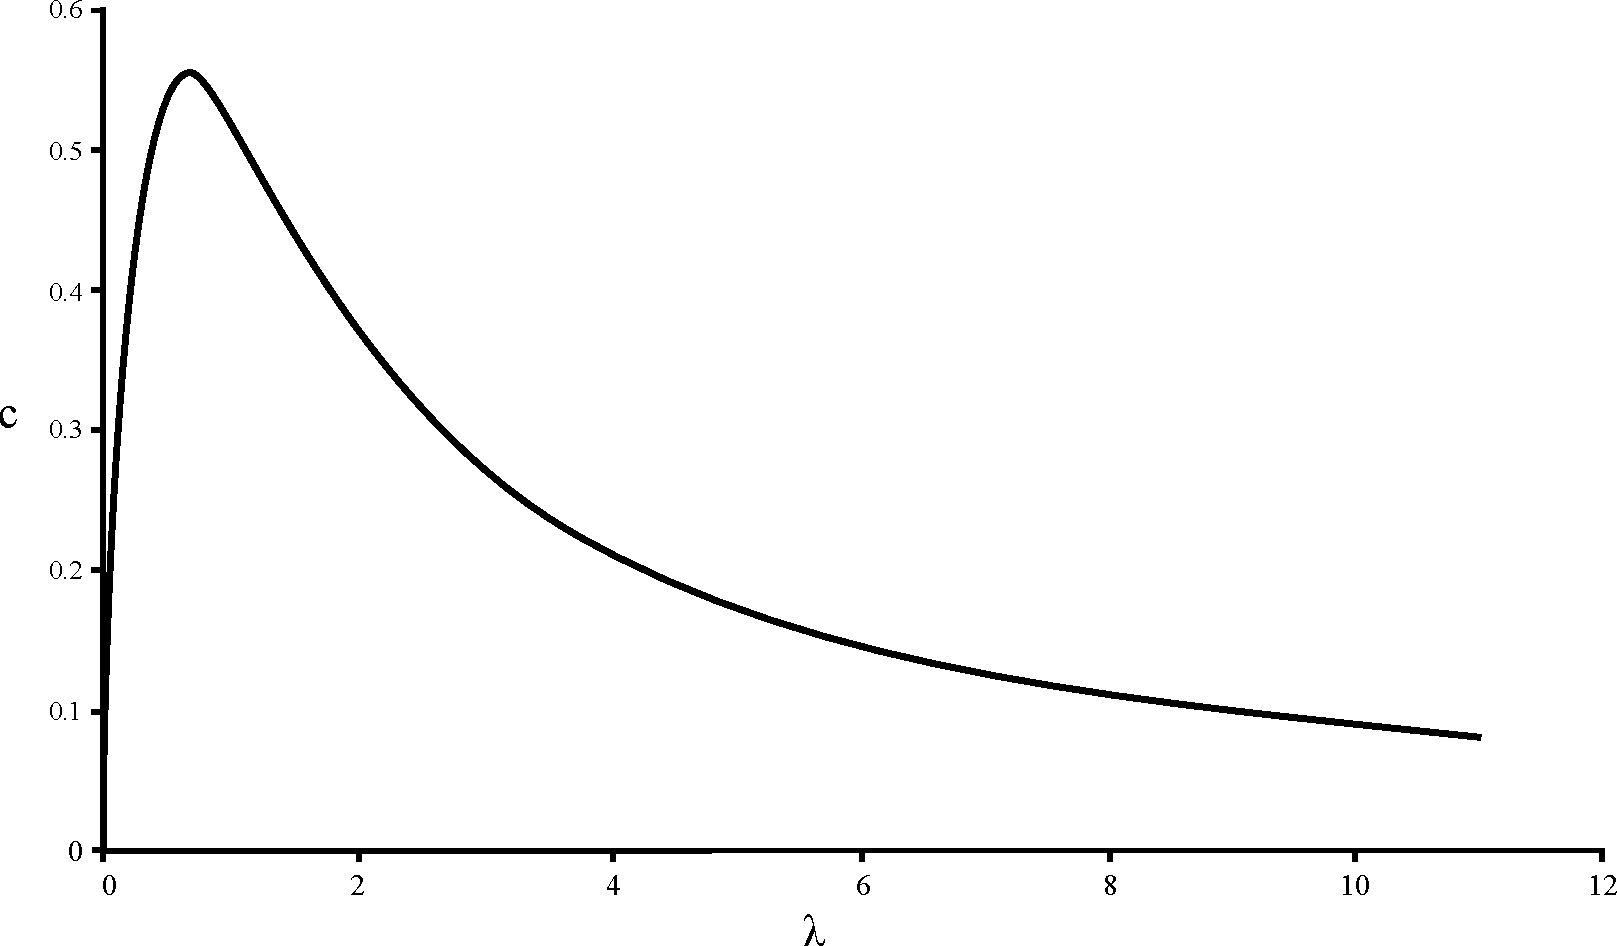
\includegraphics[width=.7\textwidth]{fig/lambdacz.pdf}
\caption{}
\label{fig:lambdacz}
\end{figure}
\subsection{Variazione della corda}
Quando si progetta una turbina lenta, nella quale $\lambda$ è compreso tra $0$ e $1$, la corda è sempre crescente. 

Quando si progetta una turbina veloce, nella quale $\lambda > 2$, la corda cresce dall'asse fino al punto nel quale $\lambda \approx 1$ e poi diminuisce fino alla periferia. 

\subsection{Relazione tra solidità, velocità specifica ed efficienza della turbina}
Se ricordiamo il concetto di solidità, definita come quoziente fra l'area delle pale e l'arena totale spazzata dal rotore, e lo esprimiamo matematicamente in forma generale, otteniamo
\begin{align*}
\sigma = \int_0^R \frac{z l }{\pi R^2} dr
\end{align*}
Poichè
\begin{align*}
\lambda_r = \frac{\Omega r}{V_1} \Rightarrow r = \frac{V_1 \lambda_r}{\Omega} \Rightarrow \frac{dr}{d \lambda_r} = \frac{V_1}{\Omega} \Rightarrow dr = \frac{V_1}{\Omega} d\lambda_r
\end{align*}
Sostituendo nell'integrale si ottiene
\begin{align*}
\sigma = \int_0^{\lambda} \frac{z l}{\pi R^2} \frac{V_1}{\Omega} d\lambda_r
\end{align*}
Possiamo moltiplicare denominatore e numeratore per alcuni fattori, in modo da accorpare variabili e costanti, senza alterare l'equazione, come segue
\begin{align*}
\sigma = \int_0^{\lambda} \frac{z l}{\pi R^2} \frac{V_1}{\Omega} \frac{\Omega C_z V_1 2 \pi}{\Omega C_z V_1 2 \pi} d \lambda_r
\end{align*}
Accorpando le costanti e portandole fuori dall'integrale
\begin{align*}
\sigma = \frac{2 \pi V_1^2}{C_z \pi \Omega^2 R^2} \int_0^{\lambda} \frac{z l \Omega C_z}{V_1 2 \pi} d \lambda_r
\end{align*}
Osservare che i termini all'interno dell'integrale corrispondono al prodotto $\sigma_l C_z \lambda_r$ e quelli all'esterno dell'integrale possono essere accorpati e semplificati come segue
\begin{align*}
\sigma = \frac{2}{C_z \lambda^2} \int_0^{\lambda} \sigma_l C_z \lambda_r d \lambda_r
\end{align*}
Possiamo risolvere numericamente questa integrale con un foglio di calcolo, assumendo, per esempio, $C_z = 0.8$ (profilo NACA 4412 con $\alpha = 5^\circ$). Si ricava il risultato che si può apprezzare nella figura \ref{fig:sigmalambda}.
\begin{figure}[h!]
\centering
  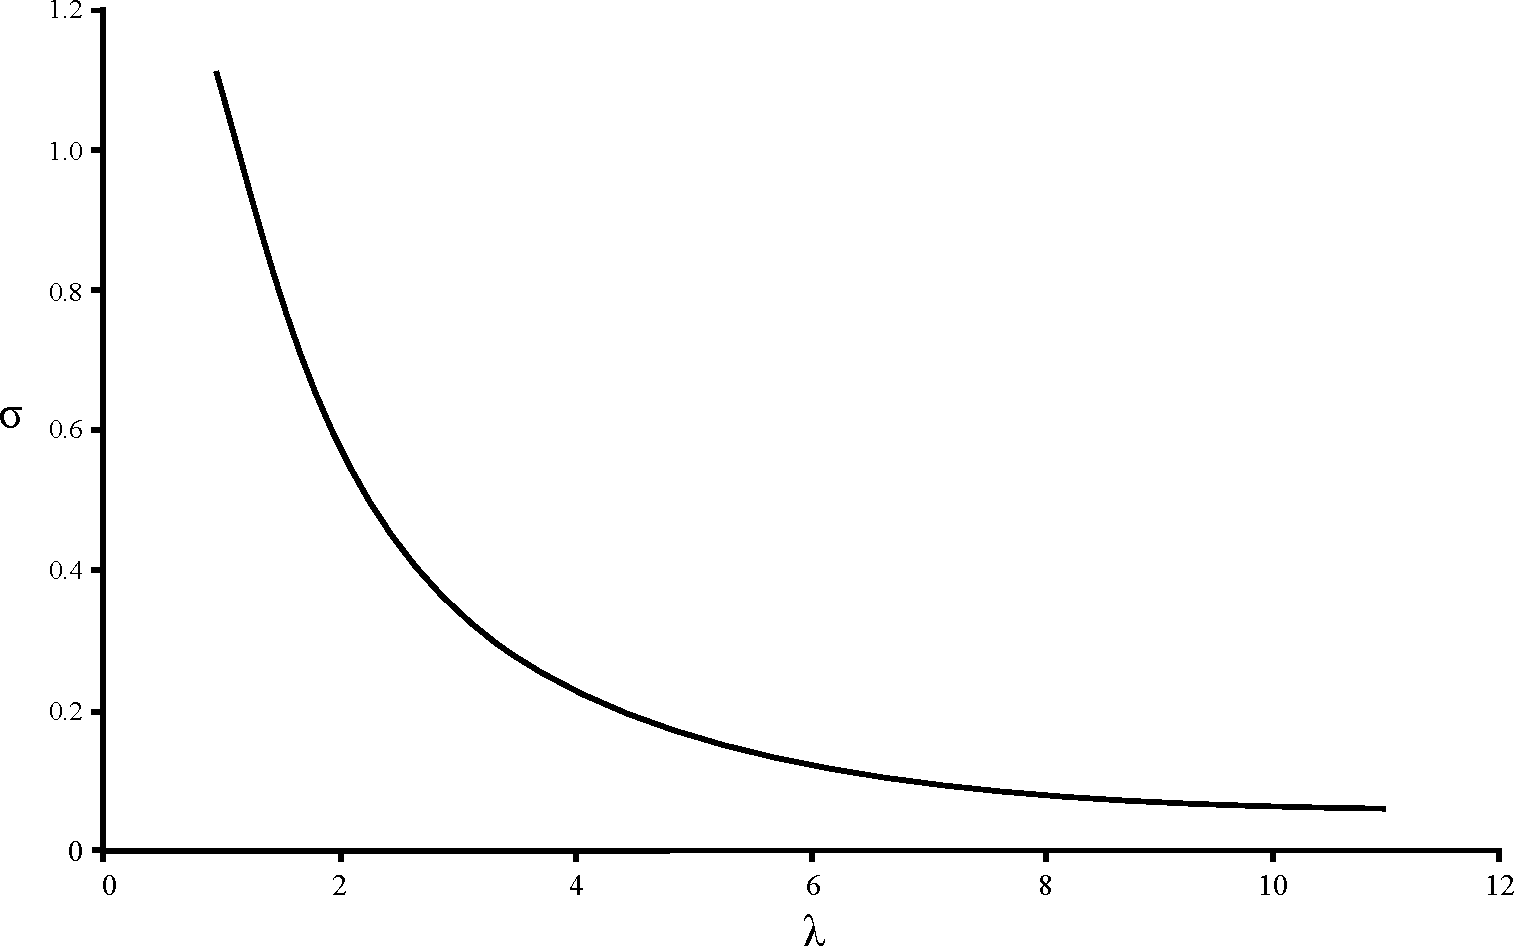
\includegraphics[width=.7\textwidth]{fig/sigmalambda.pdf}
\caption{}
\label{fig:sigmalambda}
\end{figure}
\subsection{Solidità e velocità specifica}
Dalla figura \ref{fig:sigmalambda} si evince che la solidità della turbina, $\sigma$, diminuisce con l'aumentare della velocità specifica $\lambda$. 

Nella figura \ref{fig:sigmalambda} si osserva inoltre che risulta $\sigma > 1$ per $\lambda < 1$. Questo è un risultato apparentemente contraddittorio, però non è fisicamente impossibile e spieghiamo il perché. In genere le turbine lente hanno molte pale, le quali si sovrappongono parzialmente, quindi la somma dell'area della pale può risultare maggiore dell'area spazzata dal rotore. Nella pratica però, è impossibile fare arrivare la pala fino al centro geometrico, occupato invece dal mozzo. Le turbine sono quindi caratterizzate da $\sigma \approx 1$. 

\subsection{Solidità ed efficienza aerodinamica}
Dalla Teoria di Glauert, il cui risultato si riassume graficamente nella figura \ref{fig:triangEol2}, si deduce che il coefficiente di potenza teorico, $C_p$, cresce con $\lambda$. Poiché la solidità diminuisce con $\lambda$, le macchine eoliche a bassa solidità (e quindi con un numero di pale ridotto) saranno sempre più efficienti rispetto alle macchine eoliche di alta solidità, dotate di molte pale. 

\subsection{Influenza del coefficiente di finezza del profilo}
Nello sviluppo della teoria dell'elemento di pala, abbiamo tralasciato la resistenza aerodinamica del profilo per poter ottenere le espressioni semplificate \ref{eq:dF_u2} 3 \ref{eq:dF_f2}. Questa ipotesi è abbastanza valida per i profili alari sottili, perfettamente lisci, e operanti con $Re > 500000$. Nelle reali condizioni d'esercizio (profilo di un certo spessore per garantire resistenza strutturale, superficie sporca di polvere, superficie graffiata, insetti morti, $Re < 100000$ per turbine molto piccole e venti deboli) non sempre si compie che $C_z \gg C_x$, ovverosia $f > 50$. La figura \ref{fig:cplambda} mostra come cala il coefficiente di potenza $C_p$ quando scende il coefficiente di finezza $f$. 
\begin{figure}[h!]
\centering
  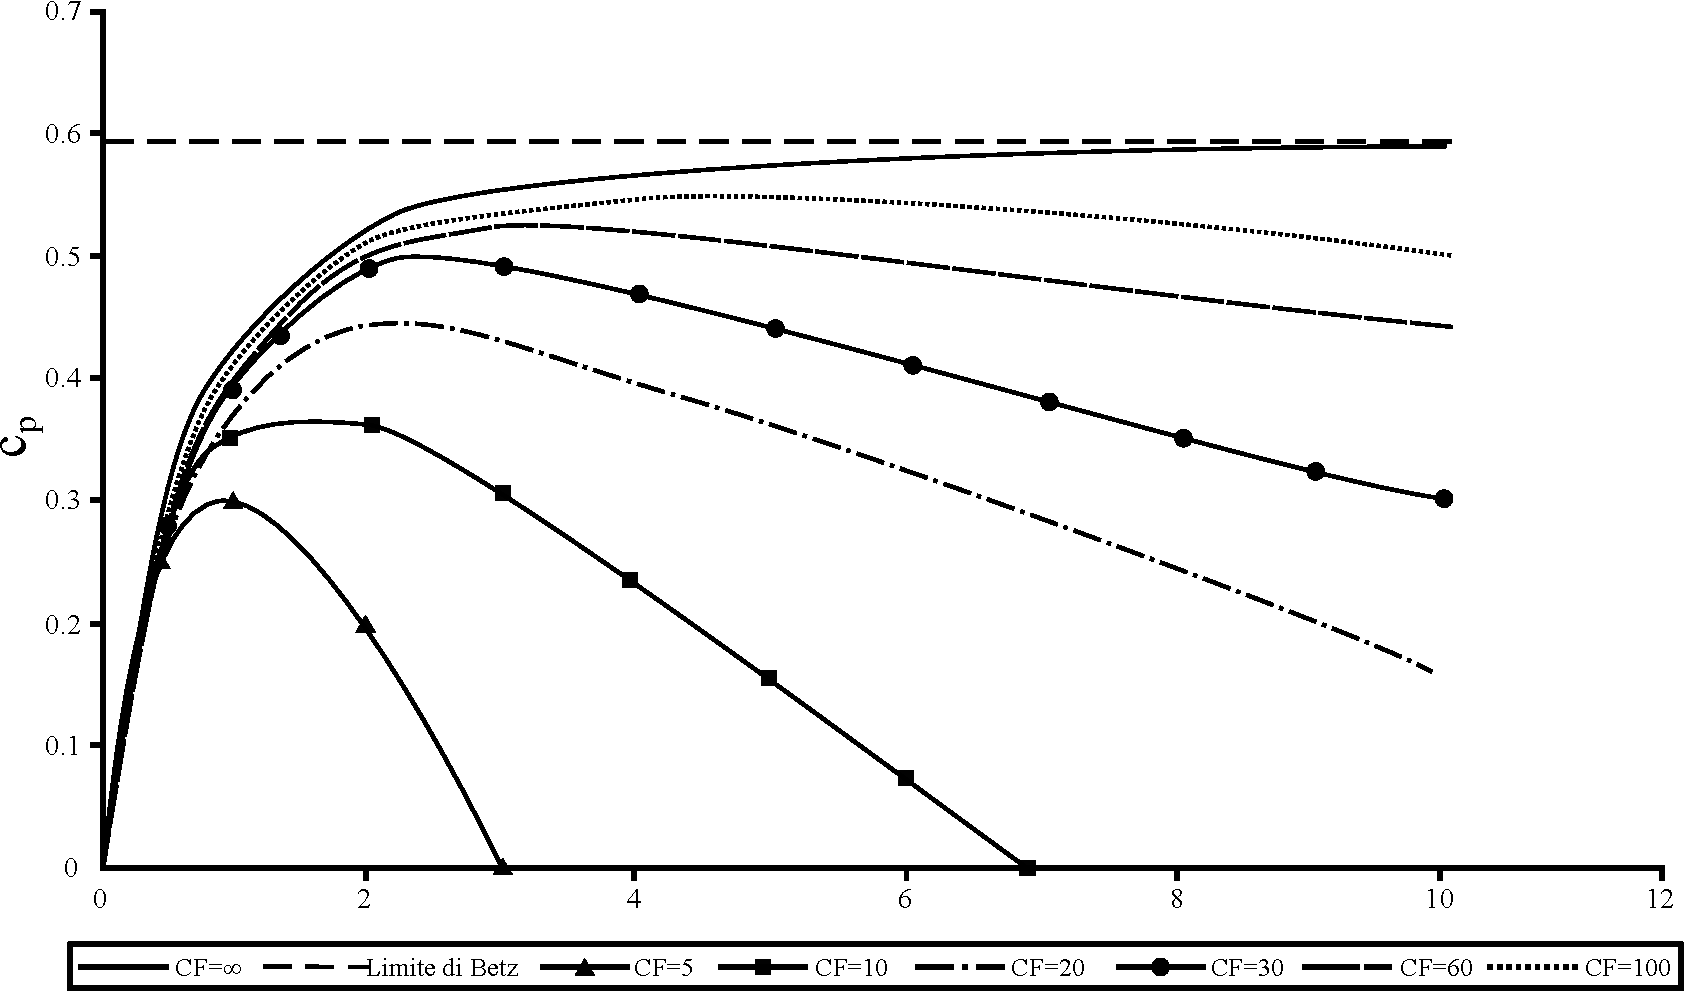
\includegraphics[width=.9\textwidth]{fig/cplambda.pdf}
\caption{}
\label{fig:cplambda}
\end{figure}

